\section{Design und Implementation}

Vor dem Umsetzen dieser Arbeit war der Vorgang zum Aktualisieren der Systeme sehr konsolenlastig. Daher war ein Ziel der Arbeit, die Applikation benutzerfreundlich und intuitiv zu gestalten. Dies wurde mit einer engen Zusammenarbeit mit den Industriepartnern sowie mit eigenen Tests und Versuchen erzielt.

\subsection*{Mockups} \label{design:mockups}

Als Diskussionsgrundlage und Vorlage für die Umsetzung wurden etwa 30 verschiedene \glspl{mockup} mit Balsamiq\footnote{\purl{https://balsamiq.com/products/mockups/}} umgesetzt. Die Wichtigsten werden hier kurz porträtiert.

\subsubsection*{Gruppierungen}

Gemäss Use-Cases 08 und 11 (siehe \ref{sec:uc_08} und \ref{sec:uc_11}) können Systeme und Pakete einer (oder mehreren für Pakete) beliebigen Gruppe zugeordnet werden. In den Entwürfen zu den entsprechenden Ansichten wurde zusätzlich zu den umgesetzten Funktionalitäten noch eine automatische Zuweisungsregel konzeptioniert. Auf Bild \ref{fig:design:group_systems_mockup} ist die Gruppe 'Test-Group' zu sehen, welcher alle neu registrierten Systeme mit 'test' im Namen automatisch zugewiesen werden. Dieses Feature wurde aber aufgrund von anderen Prioritäten nicht umgesetzt.

\begin{figure}[H]
	\centering
	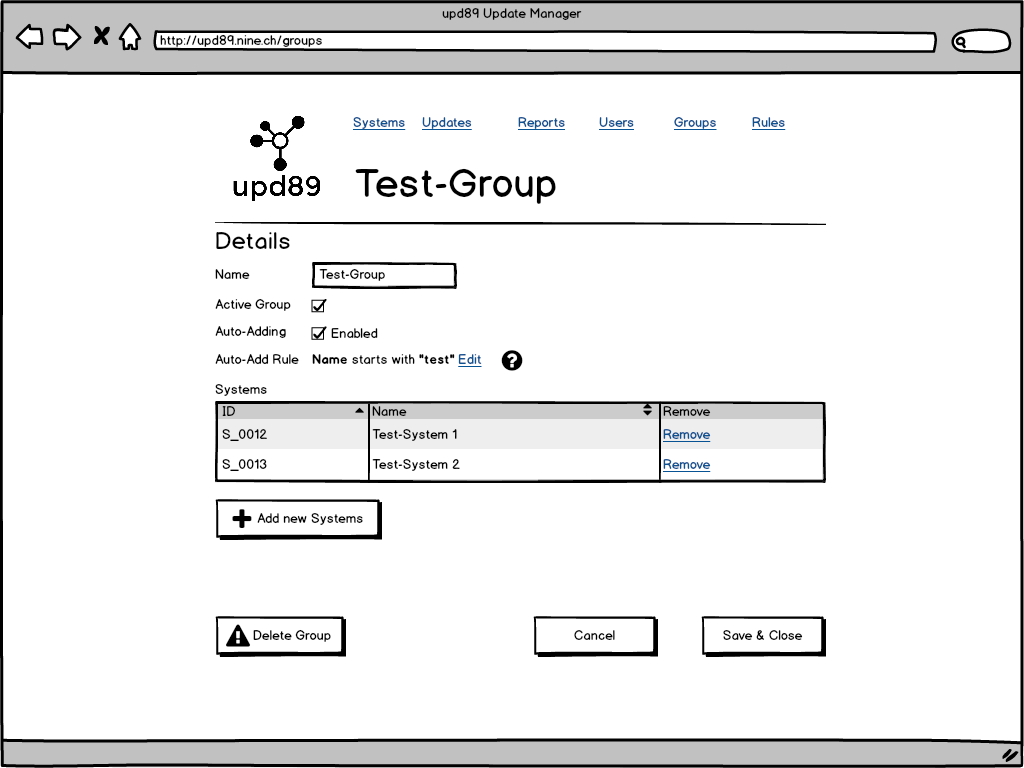
\includegraphics[width=\linewidth]{files/mockups/group_systems}
	\caption{Detail-Ansicht der Systemgruppe 'test-group'}
	\label{fig:design:group_systems_mockup}
\end{figure}

\subsubsection*{Berechtigungen} \label{sec:design:permissions}

Für den Use-Case 07 (siehe \ref{sec:uc_07}) wurden drei verschiedene Vorgehensweisen konzipiert. Die erste (Bild \ref{fig:design:permission_1}) sah vor, dass pro Benutzer die Einstellungen für jedes System, jede Art von Anwendungen und sogar unterscheidend zwischen grossen oder kleinen Versionssprüngen vorgenommen werden kann. Dies wurde aber verworfen, da der Administrationsaufwand bei Änderungen zu gross gewesen wäre. Zudem kann nicht garantiert werden, dass 'grosse' Versionssprünge korrekt erkannt werden.

Eine Alternative sah weiterhin die Verwaltung der Rechte pro Benutzer vor, aber in einer tabellarischen Form mit simplen Ja/Nein-Berechtigungen für verschiedene Aktionen (Bild \ref{fig:design:permission_2}). Hier wurde auch zwischen 'normalen' und 'kritischen' Updates unterschieden, also nur zwischen zwei Paketgruppen. Der Vorteil war die einfache Bedienung und die klare Darstellung der Berechtigungen. Aufgrund der gewünschten beliebigen Anzahl Paketgruppen wurde diese Alternative aber ebenfalls verworfen.

Schlussendlich hat sich eine Rollen- und Stufen-basierte Rechteverwaltung durchgesetzt. Jeder Benutzer wird einer Rolle zugeteilt, welche eine bestimmte Berechtigungsstufe besitzt. Ob ein Benutzer nun ein Paket auf einem System aktualisieren darf, hängt von der Gruppenzugehörigkeit des Paketes und des Systems ab.

Auf diese Weise ist es sehr einfach, ganzen Benutzergruppen die Rechte für mehrere Systeme oder Pakete auf einmal zu entziehen oder zu verteilen, was bei den alternativen Vorschlägen mindestens eine Einstellung pro User erfordert hätte.

\begin{figure}[H]
	\centering
	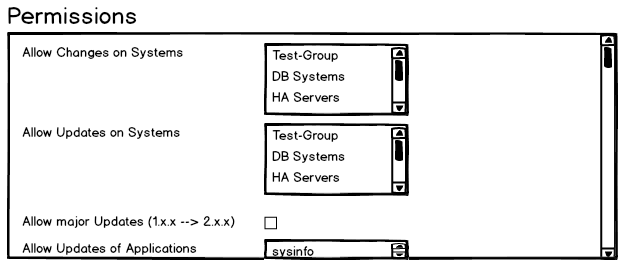
\includegraphics[width=0.75\linewidth]{files/mockups/permission_1}
	\caption{Verworfenes Rechtesystem mit verschiedenen Einstellungen}
	\label{fig:design:permission_1}
\end{figure}

\begin{figure}[H]
	\centering
	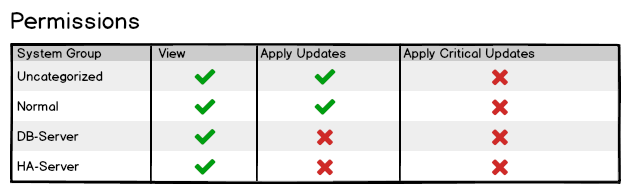
\includegraphics[width=0.75\linewidth]{files/mockups/permission_2}
	\caption{Verworfenes Rechtesystem als Tabelle mit Icons}
	\label{fig:design:permission_2}
\end{figure}

\subsubsection*{Dashboard}

Eine Art Übersichtsseite war von Beginn an geplant und auch durch den Industriepartner begrüsst. Bei einer grösseren Anzahl von Systemen ist es oft einfacher, eine vereinfachte Zusammenfassung als eine detaillierte Auflistung aller einzelnen Systeme zu lesen. Dies, sowie relevante Aktionen bei Auftreten von bestimmten Situationen anzubieten, war das Ziel des Dashboards (Abbildung \ref{fig:design:dashboard_mockup}).

Einerseits sollte sichtbar sein, wieviele Systeme verfügbar sind, auf welchen Systemen Updates anstehen oder wo gerade Installationen durchgeführt werden. Andererseits sollten auch die letzten Aktivitäten und deren Ergebnis sichtbar sein, um Probleme und deren potentiellen Ursachen schnell erkennen zu können.

Da die Funktionalität zur automatischen Zuweisung von neu registrierten Systemen und noch unbekannten Paketen in Gruppen verworfen wurde, musste dies nun manuell erledigt werden. Dazu wurde eine Auflistung dieser Systeme und Pakete auf dem Dashboard konzipiert, wo sie auch gleich in Gruppen eingeteilt werden können. 

\begin{figure}[H]
	\centering
	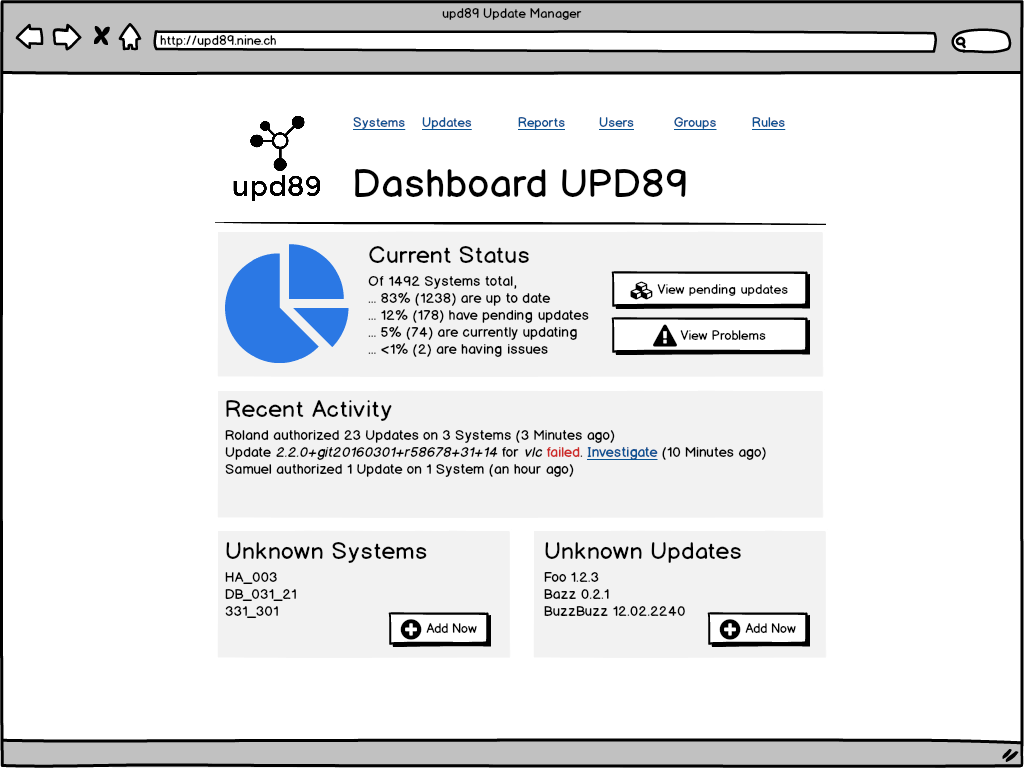
\includegraphics[width=\linewidth]{files/mockups/dashboard}
	\caption{Konzept des Dashboards}
	\label{fig:design:dashboard_mockup}
\end{figure}

\subsubsection*{System- und Paket-Ansicht}

Neben den spezifischen Ansichten für alle Pakete oder Systeme mit entsprechenden Filtern, von denen aus Updatevorgänge gestartet werden können, war es ein Wunsch des Industriepartners, auch eine kombinierte Ansicht mit Filterung und Suche nach Paketen und Systemen zu haben. Nach mehreren Entwurfsiterationen wurde schliesslich Bild \ref{fig:design:combo_view_mockup} als passendes Design gefunden. Hier ist es möglich, mehrere Pakete gleichzeitig auf mehreren, einzeln auswählbaren Systemen in Auftrag zu geben.

\begin{figure}[H]
	\centering
	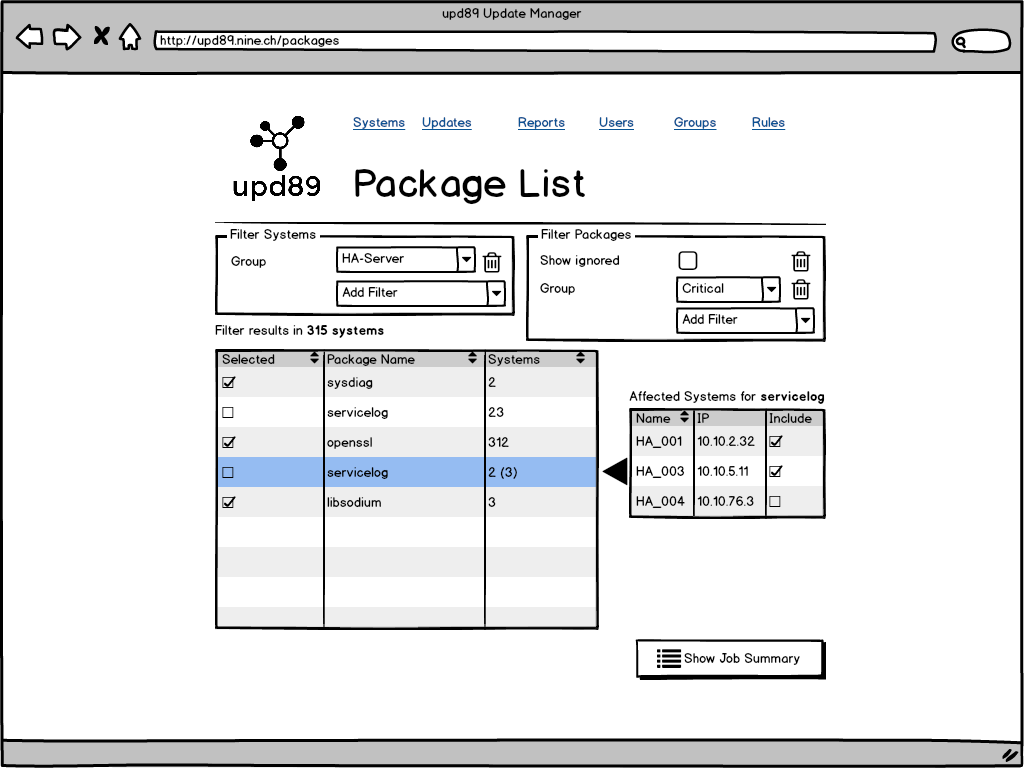
\includegraphics[width=\linewidth]{files/mockups/combo_view}
	\caption{Haupt-Ansicht mit Paket- und System-Filter}
	\label{fig:design:combo_view_mockup}
\end{figure}

\subsection*{User Interface}

Die Oberflächen halten sich grösstenteils an die Mockups aus der Planung, einige Details wurden aber aufgrund von Input durch den Industriepartner oder durch Hallway-Testing und Usability-Tests abgeändert. Siehe dazu auch das Kapitel Testing (\ref{sec:umsetzung:testing}).

\begin{figure}[H]
	\centering
	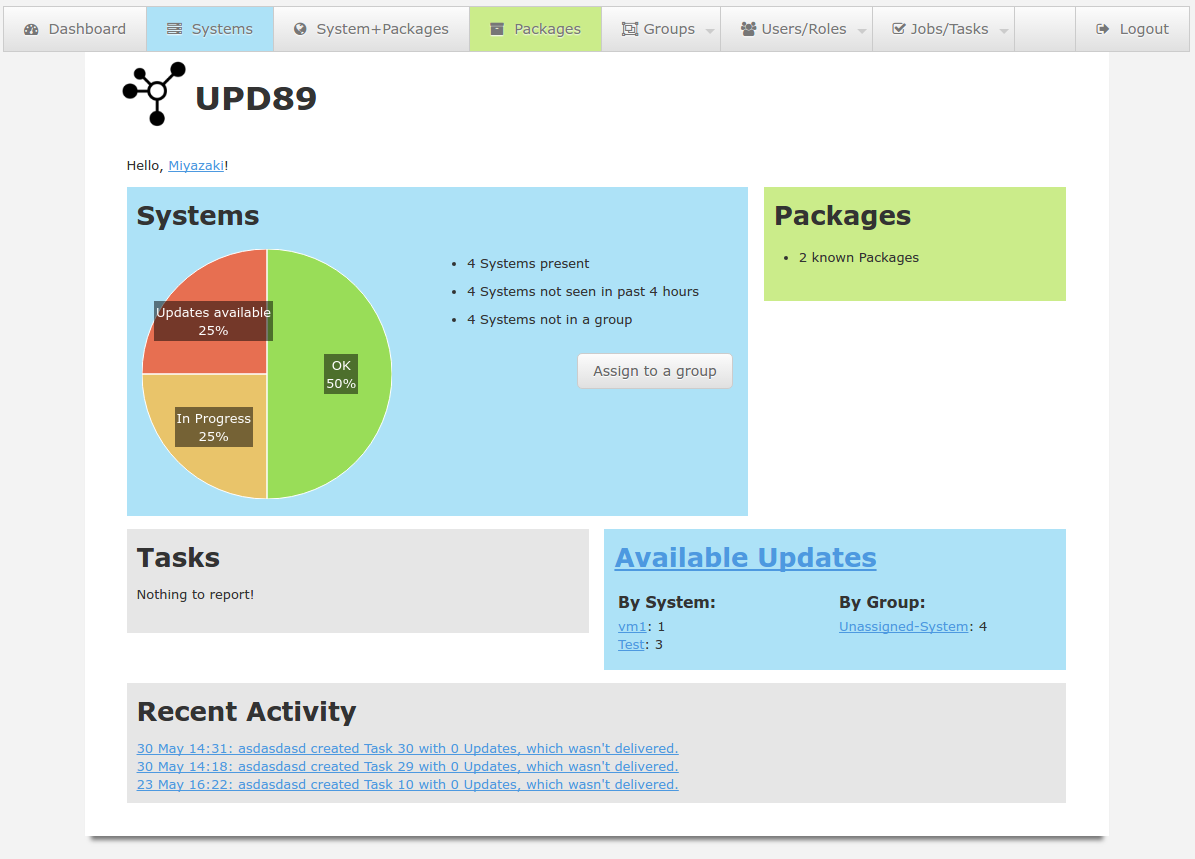
\includegraphics[width=\linewidth]{files/upd89-screenshot_dashboard}
	\caption{Umgesetztes Dashboard}
	\label{fig:design:dashboard}
\end{figure}

\subsubsection*{Javascript}

Obwohl das \gls{controlcenter} in Ruby on Rails umgesetzt wurde, spielte Javascript eine wichtige Rolle. Ohne Javascript verursacht fast jede Aktion durch den Benutzer und jede Änderung am Inhalt ein Nachladen der Seite, was je nach Inhalt und Verbindungsqualität langsam und ablenkend sein kann. 

Mit Javascript können Interaktionen des Benutzers bereits im Browser abgefangen werden und es kann darauf reagiert werden ohne den Umweg über den Server zu machen. Bei Bedarf kann der Javascript-Code aber auch Teilinhalte nachladen, ohne dass die momentane Seite verlassen werden muss. In der Paket- und System-Ansicht (Bild \ref{fig:design:js_example}) beispielsweise wird über \gls{ajax} beim Filtern von Paketen und Systemen oder auf die entsprechenden Gruppen oder beim Sortieren  der Tabellen jeweils nur der Inhalt der Tabelle neu geladen. Ein Klick auf den Pfeil neben einem Paket lädt ebenfalls via \gls{ajax} die betroffenen Systeme für die System-Tabelle auf der rechten Seite nach. Zudem wird die Schaltfläche zum Ausführen der Updates dynamisch aktiviert oder deaktiviert, je nach Auswahl von Paketen und Systemen.

\begin{figure}[H]
	\centering
	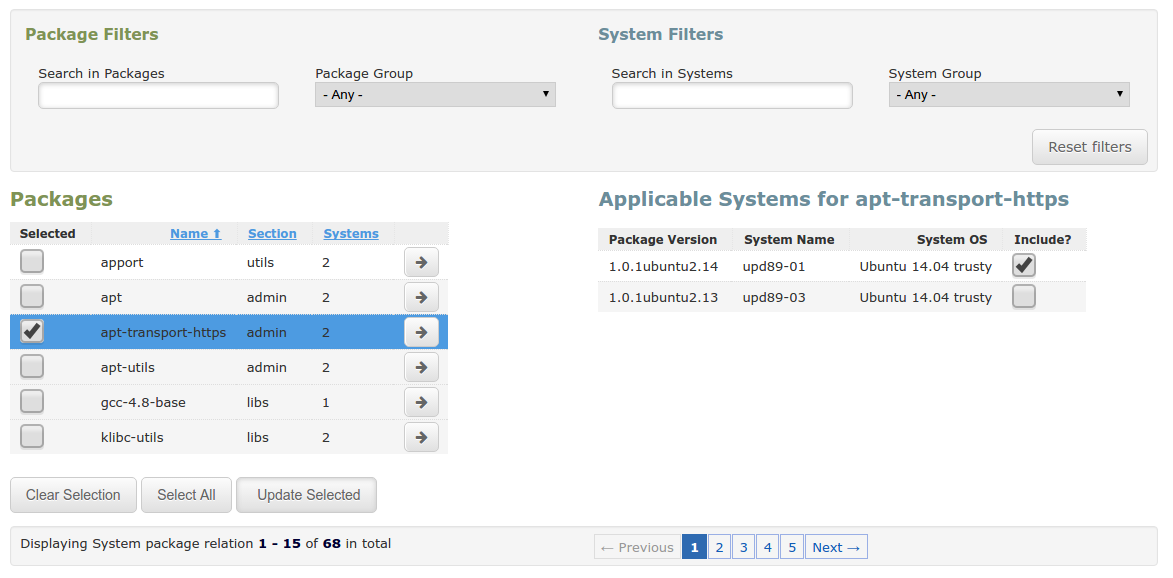
\includegraphics[width=\linewidth]{files/combo_view}
	\caption{Beispiel für Javascript-Erweiterungen des Rails-Frontends}
	\label{fig:design:js_example}
\end{figure}

\subsection*{Logo, Icon, Schriftart}

Das Logo wurde im Squarespace Logo Generator\footnote{\purl{https://www.squarespace.com/logo/}} erstellt mit dem Icon 'Nodes'\footnote{\purl{https://thenounproject.com/search/?q=nodes+by+gregor\&i=138240}} von Gregor Črešnar. Die Schriftart für 'UPD89' ist Montserrat\footnote{\purl{https://www.fontsquirrel.com/fonts/montserrat}} von Julieta Ulanovsky.

Das Icon wurde als Symbol für die zentrale Verwaltung und die Kommunikation mit den einzelnen Servern gewählt. Es kann bei Bedarf durch ein beliebiges Logo ersetzt werden.

\subsection*{Farben}

Generell wurde das Interface eher schlicht gehalten. Grautöne sowie Rot, Gelb und Grün als Signalfarben (\ref{fig:design:messages}) lassen die Seiten übersichtlich und nicht überladen erscheinen.

\begin{figure}[H]
	\centering
	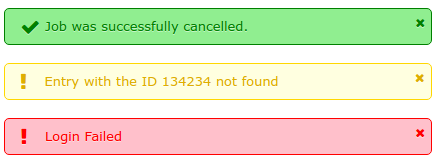
\includegraphics[width=0.5\linewidth]{files/messages}
	\caption{Beispiele der drei Hinweise 'Erfolg', 'Warnung', 'Error'}
	\label{fig:design:messages}
\end{figure}

Die selbst definierten Farben wurden in einer separaten \gls{scss}-Datei definiert, wodurch es für anwendungs- oder benutzerspezifische Anpassungen einfach abzuändern ist. Eine Übersicht über die wichtigsten Farben ist in Bild \ref{fig:design:colorcodes} zu sehen.

\begin{figure}[H]
	\centering
	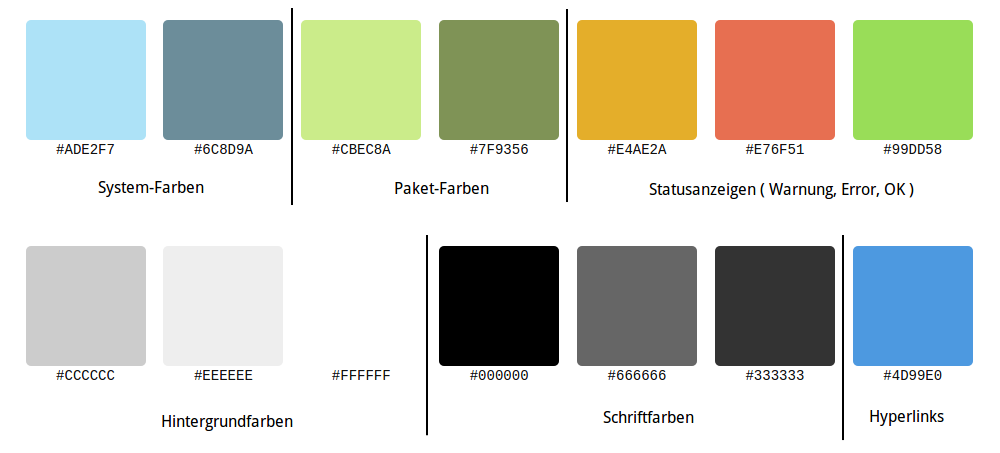
\includegraphics[width=\linewidth]{files/colorcodes}
	\caption{Verwendete Farben mit Hex-Codes}
	\label{fig:design:colorcodes}
\end{figure}

Ein besonderes Augenmerk wurde auf die farbliche Kennzeichnung der Systeme und Pakete gelegt. Besonders in der kombinierten Ansicht, wo es Filtermöglichkeiten zu Systemen und zu Paketen gibt, ist es mit einer farblichen Unterscheidung einfacher zu sehen, was welche Entitätsgruppe betrifft. Diese Farben wurden auch ins Menu und ins Dashboard weitergezogen; in der ganzen Applikation sind Infos und Einstellungen, welche für Systeme relevant sind, generell im 'System-Blau' und solche für Pakete im 'Paket-Grün' (Beispiel im Bild \ref{fig:design:sys_pkg_colors}).

\begin{figure}[H]
	\centering
	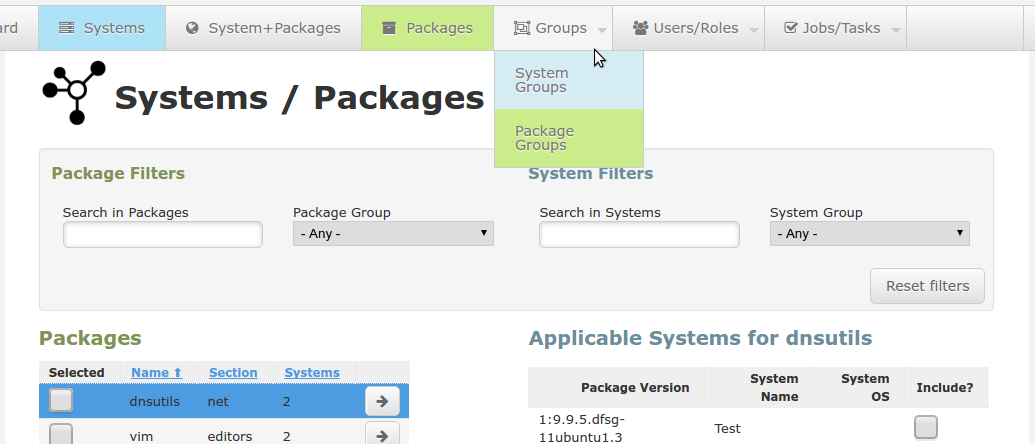
\includegraphics[width=\linewidth]{files/colors_pkg_sys}
	\caption{Farb-Hinweise: Blau für Systeme, Grün für Pakete}
	\label{fig:design:sys_pkg_colors}
\end{figure}

\subsubsection*{Building Blocks}

Um verschiedene grafische Elemente konsistent gleich aussehen zu lassen, wurde das HTML Kickstart-Framework von Joshua Gatcke/99lime.com\footnote{\purl{http://www.99lime.com/elements/}} verwendet. Dadurch waren gewisse Funktionalitäten wie etwa das Menu oder die Hinweise bereits vorhanden.

Für die Icons wurde FontAwesome\footnote{\purl{http://fontawesome.io/}} verwendet.

\subsection*{Regelwerk}

\begin{decision}{Regelwerk}
Die Anforderung bezüglich einem Regelwerk aus der Aufgabenstellung wurde während des Projekts in Absprache mit den Projektpartnern gestrichen. Die Funktionalität wurde als zu komplex erachtet und andere Features wurden höher priorisiert. Jedoch wurden Vorschläge und Mockups erstellt, wie in Kapitel \ref{sec:ausblick:regelwerk} ersichtlich ist.
\end{decision}
